\documentclass[10pt]{article} 
\usepackage{a4} 
\usepackage{makeidx}
\usepackage[danish]{babel} 
\usepackage[utf8]{inputenc}
\usepackage{textcomp}
\usepackage{amsmath}
\usepackage{amssymb}
\usepackage{amsthm}
\usepackage{graphicx} 
\usepackage{verbatim} 
\usepackage{fancyhdr}
\usepackage{listings} 
\usepackage{url}
\frenchspacing
\makeindex
\pagestyle{plain}
\newcommand{\Oh}[0]{ \mathcal{O} }
%\addtolength{\voffset}{-70pt}
%\addtolength{\textheight}{70pt}

%\addtolength{\hoffset}{-40pt}
%\addtolength{\textwidth}{80pt}

\lstset{language=Python}
\title{Grundlæggende Datalogi -- Introdag}
\author{RasmusJensen@kommunikationogit.dk}
\date{27/8 2009}

\begin{document}

\maketitle

\section{Plan for i dag}
\begin{itemize}
\item Introduktion til kurset Grundlæggende Datalogi
\item Installér JES
\item Leg med Python
\end{itemize}

\section{Installation af JES}
... om programmering, 
-
overblik over programmet
\begin{center}
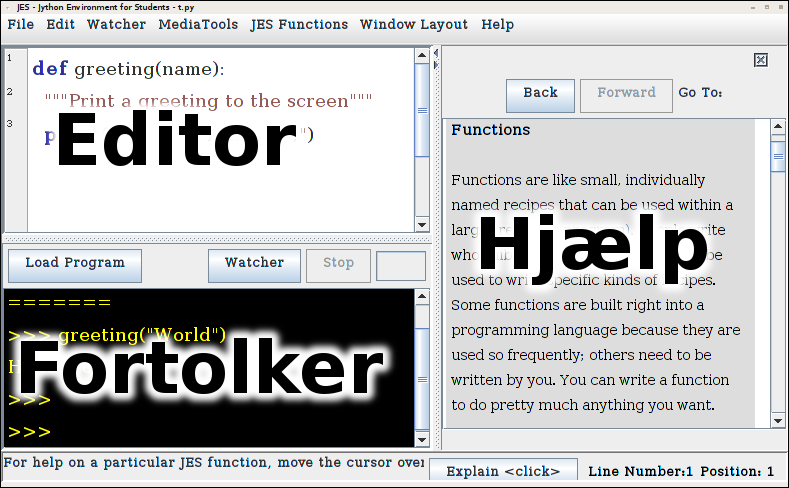
\includegraphics[width=300pt]{JESdesc.png}
\end{center}
\section{I gang med Python}
\subsection{Kald af funktioner}

\subsection{Regnemaskine og tekst}
\paragraph{Øvelse:} Prøv at bruge fortolkeren som en lommeregner
\subsection{Debugging}
... følsomhed for korrekt syntaks
... eksperimenter i fortolkeren
... ikke danske bogstaver
\subsection{Variable (navngivning)}
\paragraph{Eksempel:} 


\verbatiminput{smiley.py}


\end{document}

